\begin{frame}[parent={cmap:software-testing-foundations}, hasprev=false, hasnext=true]
\frametitle{Defect taxonomy}
\framesubtitle{Fault}
\label{concept:fault}

\begin{block:concept}{What is a fault?}
A fault is an incorrect data definition, step, or process in a software.
\end{block:concept}

\begin{block:fact}{How a fault is created?}
\begin{itemize}
	\item A fault is inserted by a mistake.
\end{itemize}
\end{block:fact}

\hfill
\refie{example:incorrect-statement-2}{\beamerbutton{Example: Incorrect statement}}
\end{frame}



\begin{frame}[hasprev=true, hasnext=true]
\label{concept:mistake}
\frametitle{Defect taxonomy}
\framesubtitle{Mistake}

\begin{block:concept}{What is a mistake?}
A mistake is a human action that produces an incorrect result.
\end{block:concept}

\begin{block:fact}{How a mistake takes place?}
\begin{itemize}
	\item Lack of attention when implementing the software?

	\item Omitted information in the software requirement specification?

	\item Compiler fault (which by itself was caused by a mistake)?
\end{itemize}
\end{block:fact}

\hfill
\refie{example:incorrect-statement-1}{\beamerbutton{Example: Incorrect statement}}
\end{frame}



\begin{frame}
\label{concept:error}
\frametitle{Defect taxonomy}
\framesubtitle{Error}

\begin{block:concept}{What is an error?}
An error is the difference between a computed, observed or measured value
or condition and the true, theoretically correct or specified value or
condition.
\end{block:concept}

\begin{block:fact}{How an error occurs?}
\begin{itemize}
	\item An error is produced by the execution of a fault.
	\begin{itemize}
		\item Thus, if a fault is never executed, it never produces an error.
	\end{itemize}
\end{itemize}
\end{block:fact}
\end{frame}


\begin{frame}
\label{concept:failure}
\frametitle{Defect taxonomy}
\framesubtitle{Failure}

\begin{block:concept}{What is a failure?}
A failure is the inability of a component or a system to fulfill its
required functions within specified performance requirements.
\end{block:concept}

\begin{block:fact}{How a failure occurs?}
\begin{itemize}
	\item A fault and its associated errors may cause one or more failures.
\end{itemize}
\end{block:fact}

\hfill
\refie{example:incorrect-statement-3}{\beamerbutton{Example: Incorrect statement}}
\end{frame}



\begin{frame}
\frametitle{Defect taxonomy}

\begin{block:procedure}{Summary}
\begin{enumerate}
	\item A programmer makes a \textbf{mistake}.
	\begin{itemize}
		\item One single $<$ is replaced by a $>$ in a single statement.
	\end{itemize}

	\item Due to the mistake, the statement is \textbf{faulty} (it does
	not implement the behavior described in the software requirements
	specification).

	\item The software is compiled and run. The given statement is run. As it
	belongs to a function in charge of creating the checksum of the data being
	processed, the output is produces is incorrect (\textbf{error}).

	\item The user compares the checksum produces by the software with the
	expected one. No matter what, the checksum always \textbf{fails}.
\end{enumerate}
\end{block:procedure}
\end{frame}



\begin{frame}[c, hasprev=true, hasnext=false]
\label{concept:defect-taxonomy}
\frametitle{Defect taxonomy}

\begin{block:fact}{}
    \centering
    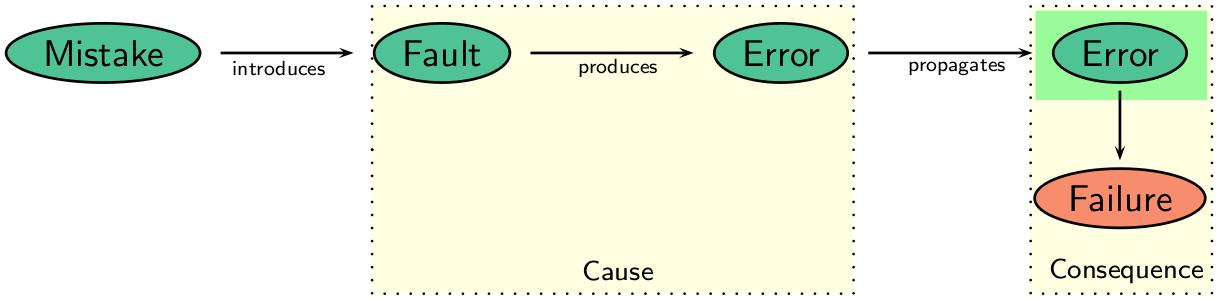
\includegraphics[scale=.3]{defect-taxonomy}
\end{block:fact}

\hfill
\refie{example:physician-analogy-for-defect-taxonomy}{\beamerbutton{Example: Physician analogy for defect taxonomy}}
\refie{example:numzero}{\beamerbutton{Example: Defect taxonomy example (numZero)}}
\end{frame}
